\subsection{Hardware details and safety features}
CALIS offers various safety features to ensure that the device runs smoothly, no components are lost inside the detector, avoid any contamination of the detector by dirty or incompatible materials, maintain pressure and avoid introduction of oxygen or water in contact with the LS and TMB. %, operation in the volume that excludes possibility of contact with PMTs or light pulsers (pacman) attached to each PMT.

\begin{description}

\item[Drive mechanism:]
In the event of a power failure, the magnetic break ensures there is no movement of the pig. The torque of the servo motor is limited in case of an unexpected load. 

The speed reducer (gears) is a double worm gear design. The primary worm gear has a 50:1 reduction and the secondary worm has a 82:1 reduction. The input speed of the servo motor is 2400 RPMs and the output is 0.6 RPM and has the weight capacity of 148 lbs. In the event of a power failure the speed reducer has the ability to hold the load at any position without back drive. The speed of the motor has been limited to 0.4\,cm/s which minimizes any lateral oscillation of the pig during lowering and raising the source. Additionally, this is the maximum speed at which the motor is not overheating.


\item[Cable strength:]
The cables holding the pig have been rated for loads over 590\,kg, while the weight of the deployment device is at the level of 10-15\,kg so well below the breaking strength of the cable. 

\item[Cable length:]
The cable length has been established so that the maximum depth at which the pig can be deployed is above the level of the PMTs inside the LSV. In case, the command is given to deploy to greater depth, the cable completely unwinds and then rewinds in the opposite direction, which then effectively retracts the pig to a higher z-position until the preset motor count of steps is reached. 

\item[Manual retraction system:]
In the unlikely case of a complete motor failure while the source is deployed, it is possible to manually retract the pig back to its home position and close the gate valve. The motor is disengaged, and wrench is used to manually wind the cable back onthe spools and retract the pig back above the gate valve. 
   
\item[High limit switch:]
A high limit switch is a hardware interlock, that prevents the deployment device to hit the cable spools and gears, should it pass beyond the home position in the CALIS housing (Fig.~\ref{fig:CALISMechanism}). 

\textit{Neither the manual retraction system had to be used so far nor has the high limit switch been activated during calibration campaigns.}
    
\item[Light and leak tightness of CALIS:]
When the deployment device is next to the cryostat the gate valve is open and we take also data with the LSV. A prerequisite is that the housing is absolute light tight and pressure leak tight. All view ports have light tight covers for when the organ pipe gate valve is open. Both light and leak tightness has been extensively validated throughout the manufacturing process until including commissioning (Sec.~\ref{sec:Commissioning}).

\item[Securing of the source]
All connection points for the source and arm have been secured with two push locking pins that cannot be disengaged without a person pressing the pin (Fig.~\ref{fig:sourceHolder_locking}). In addition, the source holder and the two locking pins will all be tethered from outside the view port until they are locked in place eliminating the possibility of accidental falling into the inside of the CALIS housing.

\end{description}
	
%%%%%%%%%%%%%%%%%%%%%%%%%%%%%%%%%%%%%%%%%
%%%%%%%%%%%%%%%%%%%%%%%%%%%%%%%%%%%%%%%%%

\begin{figure}[htbp]
 \centering
 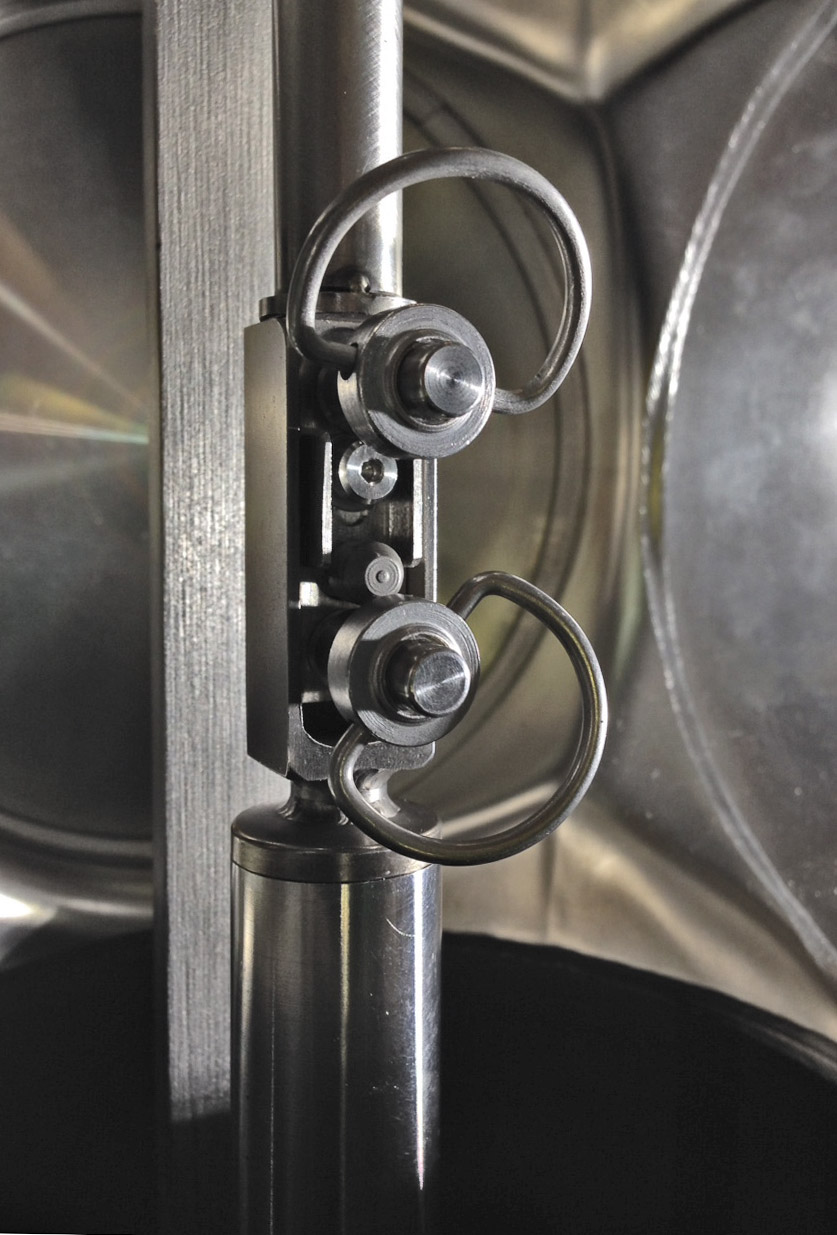
\includegraphics[width=0.3\textwidth]{Figures/sourceHolder_locking}
 \caption{Locking mechanism for the source holder. This photo shows two push pins that ensure that the sliding pin stays in place and the source holder cannot under any circumstances get detached from the arm.  The only way to remove the push pins is to depress buttons on each of them by hand.}
 \label{fig:sourceHolder_locking}
\end{figure}

%\begin{figure}[htbp]
% \centering
 % \includegraphics[width=7in]{Figures/sourceAttachmentParts}
%  \caption{Components of the source attachment mechanism. Central image shows how the pin that holds the source holder slides down and prevents the %source from getting loose.  The slide pin is locked in place by two push pins shown in Fig. \ref{fig:sourceHolder_locking}}
%  \label{fig:sourceAttachmentParts}
%\end{figure}
